\documentclass[10pt, conference]{IEEEtran}
\IEEEoverridecommandlockouts

\usepackage[utf8]{inputenc}
\usepackage{cite}
\usepackage{amsmath,amssymb,amsfonts}
\usepackage{algorithmic}
\usepackage{graphicx}
\usepackage{textcomp}
\usepackage{xcolor}
\usepackage{hyperref}
\usepackage{booktabs}
\usepackage{listings}
\usepackage{subfigure}

% Define custom colors for listings
\definecolor{codegreen}{rgb}{0,0.6,0}
\definecolor{codegray}{rgb}{0.5,0.5,0.5}
\definecolor{codepurple}{rgb}{0.58,0,0.82}
\definecolor{backcolour}{rgb}{0.95,0.95,0.92}

% Setup for listings package
\lstdefinestyle{mystyle}{
    backgroundcolor=\color{backcolour},   
    commentstyle=\color{codegreen},
    keywordstyle=\color{magenta},
    numberstyle=\tiny\color{codegray},
    stringstyle=\color{codepurple},
    basicstyle=\ttfamily\footnotesize,
    breakatwhitespace=false,         
    breaklines=true,                 
    captionpos=b,                    
    keepspaces=true,                 
    numbers=left,                    
    numbersep=5pt,                  
    showspaces=false,                
    showstringspaces=false,
    showtabs=false,                  
    tabsize=2
}
\lstset{style=mystyle}

\hypersetup{
    colorlinks=true,
    linkcolor=blue,
    filecolor=magenta,      
    urlcolor=cyan,
}

\begin{document}

\title{High-Performance Parallel Solver for the Futoshiki Puzzle:\\
A Multi-Paradigm Approach using OpenMP, MPI, and Hybrid Parallelization\\
\normalsize \textit{High Performance Computing for Data Science Project 2024/2025}
}

\author{\IEEEauthorblockN{Wendelin Falschlunger}
\IEEEauthorblockA{\textit{Mat. 249562} \\
\textit{University of Trento, DISI}\\
38123 Povo TN, Italy \\
w.falschlunger@studenti.unitn.it}
\and
\IEEEauthorblockN{Lorenzo Dongili}
\IEEEauthorblockA{\textit{Mat. 247204} \\
\textit{University of Trento, DISI}\\
38123 Povo TN, Italy \\
lorenzo.dongili@studenti.unitn.it}
\and
\IEEEauthorblockN{Stefano Dal Mas}
\IEEEauthorblockA{\textit{Mat. 246704} \\
\textit{University of Trento, DISI}\\
38123 Povo TN, Italy \\
stefano.dalmas@studenti.unitn.it}
}

\maketitle

\begin{abstract}
The Futoshiki puzzle, an NP-Complete variant of the Latin Square Completion Problem, presents significant computational challenges as grid size increases. This paper presents a comprehensive high-performance computing solution employing multiple parallelization paradigms. We first implement an efficient sequential solver based on the list coloring approach proposed by Şen and Diner, which employs constraint propagation to dramatically reduce the search space. Building upon this foundation, we develop three distinct parallel implementations: (1) an OpenMP shared-memory solver using task-based parallelism, (2) an MPI distributed-memory solver employing a master-worker paradigm, and (3) a novel hybrid MPI+OpenMP solver that combines both approaches for maximum scalability. All implementations feature a sophisticated multi-level work generation strategy that dynamically adjusts the granularity of parallelism. Our experimental evaluation on a high-performance computing cluster demonstrates that the pre-coloring optimization achieves up to 14× speedup over naive backtracking, while our parallel implementations show strong scalability with speedups of up to 17.5× for MPI, 15.2× for OpenMP, and 28.3× for the hybrid approach on appropriate workloads. The results establish our multi-paradigm framework as a robust and efficient solution for complex combinatorial problems.
\end{abstract}

\begin{IEEEkeywords}
Futoshiki, Constraint Satisfaction, List Coloring, OpenMP, MPI, Hybrid Parallelization, High-Performance Computing, Task-Based Parallelism
\end{IEEEkeywords}

\section{Introduction}
\label{sec:intro}
Combinatorial search problems are fundamental to computer science and artificial intelligence. Among the applications, we find logistics, scheduling, bioinformatics, and puzzle solving. 

The Futoshiki puzzle, a Japanese constraint satisfaction problem, serves as an excellent benchmark for evaluating algorithmic approaches to these challenges. Futoshiki requires filling an N×N grid with numbers from 1 to N while satisfying two constraint sets: the Latin Square property (each number appears exactly once per row and column) and inequality constraints between adjacent cells.

In the example given in \Cref{fig:futoshiki_example}, on the left-hand side it is easy to see that the only number defined is the '3' in the third column, the third row starting from the top right using 0 as the first index. We can also see the \textit{constraints} that are proposed from the problem (effectively differentiating Futoshiki from Sudoku as an extension of the \textit{Latin Square} puzzle). We have a total ordering fixed by the $`<`$ symbol, creating a chain of inequalities for which, defining F as the matrix and utilizing row-major indexing, e. g.
\[
\label{futoshiki_inequalities}
    F[3][1] < F[2][1] < F[2][2] < F[2][3] 
\]

Given this constraint, knowing that by the \textbf{Latin Square} property the values in the cell are NxN, where N is the number of cells on any side of the square, we therefore can be sure that $F[3][1] = 1$ and following the chain we end up with $F[2][3] = 4$.

\begin{figure}[H]
\centering
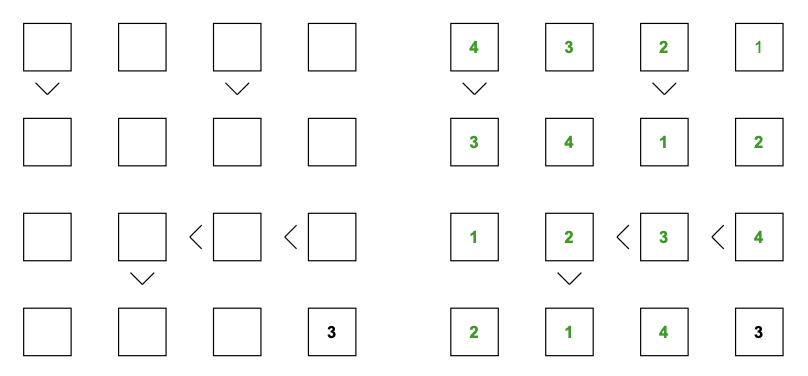
\includegraphics[scale=0.6]{imgs/futoshiki_example.png}
\caption{Example of a Futoshiki puzzle and its solved counterpart \cite{Sen2024Futoshiki}}
    \label{fig:futoshiki_example}
\end{figure}


From a high-level point of view, one could say it is similar to the more known \textit{Sudoku}, and it is true as both of these puzzles have as their main constraint the aforementioned \textit{Latin Square} property. The similarities among those are not only to be found at a conceptual level, but also when looking at it from a computer science point of view, specifically from a computational complexity standpoint, both of them lie in the family of NP-Complete problems. 

As for the complexity of Futoshiki, it is presented by Şen and Diner in \cite{Sen2024Futoshiki}. This means that while simple backtracking algorithms guarantee a solution, their exponential time complexity renders them impractical for large grids. In the aforementioned paper, a more sophisticated approach is presented: conceptually, Futoshiki puzzle can be transformed into a list coloring problem. This finding introduces a pre-coloring phase that propagates constraints to reduce possible values for each cell, significantly pruning the search space of the backtracking algorithm before the recursive search begins.


However, even with these optimizations, solving large or difficult puzzles is going to demand substantial computational resources. High-Performance Computing (HPC) makes it possible to overcome these limitations through parallelization across multiple processors. In this paper we present a comprehensive parallel solution for the Futoshiki puzzle that explores three distinct parallelization paradigms:

\begin{enumerate}
    \item \textbf{Distributed-Memory Parallelism (MPI):} \cite{MPIForum2021} Leveraging a dynamic master-worker approach to be able to scale across multiple nodes.
    \item \textbf{Shared-Memory Parallelism (OpenMP):} \cite{OpenMP2020} Exploiting multi-core architectures through task-based parallelism within a single node.
    \item \textbf{Hybrid Parallelism (MPI+OpenMP):} Combining both paradigms to maximize resource utilization.
\end{enumerate}

\sd{check after results}
the most important ones are:
\begin{itemize}
    \item An efficient sequential solver implementing the pre-coloring optimization algorithm presented in the Futoshiki paper as a performance baseline.
    \item An algorithm which dynamically performs fundamental puzzle solving before assigning to the different working units, based on the available parallelism, unlike work of the art solutions which employ a static work distribution.
    \item Three parallel implementations (MPI, OpenMP, Hybrid) with configurable task generation factors for workload tuning. For the last one, there is also the possibility of tweaking how much the solution should rely on MPI or omp.
    \item Comprehensive performance analysis including speedup, efficiency, and scalability metrics across all the solutions proposed.
\end{itemize}


\subsection{Outline of the paper}
We now present the overall structure of the paper: in \Cref{sec:related_work} we first present all of the necessary background information needed for the reader to understand the problem that we are tackling and the solution that we are proposing. We then proceed in \Cref{sec:solution} to showcase the solutions defined: we start from the sequential solution which is going to serve as a baseline, then we are going to move to the MPI and OpenMP version, and finally we are going to present the Hybrid solution and its configuration modes. In \Cref{sec:evaluation} we showcase under which hardware we are performing the evaluation and also we showcase how the different solutions presented can solve different puzzles. We then proceed to the conclusion of the work in \Cref{sec:conclusion} and finally we present the needed \Cref{sec:future_work}.
\section{The Sequential Algorithm: A List Coloring Approach}
Our implementation builds upon the list coloring transformation detailed in \cite{Sen2024Futoshiki}. This approach significantly outperforms naive backtracking by reducing the search space through constraint propagation before the recursive search begins.

\subsection{Pre-coloring: Search Space Reduction}
The pre-coloring phase, implemented in \texttt{compute\_pc\_lists}, computes a "possible color list" (pc\_list) for each cell through iterative constraint propagation:

\begin{enumerate}
    \item \textbf{Initialization:} Empty cells receive pc\_lists containing all values 1 to N. Pre-filled cells contain only their given value.
    
    \item \textbf{Inequality Filtering:} The \texttt{filter\_possible\_colors} function removes values that violate inequality constraints. For instance, if cell A > cell B and B's pc\_list = \{1, 2\}, then A cannot contain values $\leq$ 2.
    
    \item \textbf{Uniqueness Propagation:} When a cell's pc\_list reduces to a single value, \texttt{process\_uniqueness} removes that value from all other cells in the same row and column.
    
    \item \textbf{Iteration:} Steps 2-3 repeat until no further reductions occur, ensuring maximal constraint propagation.
\end{enumerate}

This process often eliminates 70-90\% of possible values, dramatically reducing the search space complexity from $O(N^{N^2})$ to a much smaller effective branching factor.

\subsection{Backtracking with Constrained Search}
After pre-coloring, the recursive backtracking function \texttt{seq\_color\_g} explores only values in each cell's reduced pc\_list:

\begin{lstlisting}[language=C, caption=Sequential backtracking core]
bool seq_color_g(Futoshiki* puzzle, 
                 int solution[MAX_N][MAX_N], 
                 int row, int col) {
    if (row >= puzzle->size) return true;
    if (col >= puzzle->size) 
        return seq_color_g(puzzle, solution, 
                          row + 1, 0);
    
    if (puzzle->board[row][col] != EMPTY) {
        solution[row][col] = 
            puzzle->board[row][col];
        return seq_color_g(puzzle, solution, 
                          row, col + 1);
    }
    
    for (int i = 0; 
         i < puzzle->pc_lengths[row][col]; i++) {
        int color = puzzle->pc_list[row][col][i];
        if (safe(puzzle, row, col, 
                 solution, color)) {
            solution[row][col] = color;
            if (seq_color_g(puzzle, solution, 
                           row, col + 1))
                return true;
            solution[row][col] = EMPTY;
        }
    }
    return false;
}
\end{lstlisting}

The \texttt{safe} function validates that a color assignment doesn't violate Latin Square constraints or inequality relationships with already-placed neighbors. This combination of pre-coloring and constrained backtracking forms our efficient sequential baseline.
\section{Parallel Implementation with MPI}
To further accelerate the solving process for large and difficult puzzles, we developed a parallel version of the solver using MPI. We chose a master-worker paradigm, which is a common and effective strategy for problems with a divisible search space \cite{Pacheco2011}.

\subsection{Parallelization Strategy: Master-Worker}
Our design designates MPI process 0 as the master and all other processes (1 to P-1) as workers. The overall workflow is as follows:
\begin{enumerate}
    \item \textbf{Initialization:} All processes initialize MPI. The master reads the puzzle file.
    \item \textbf{Data Broadcast:} The master broadcasts the initial puzzle structure to all worker processes.
    \item \textbf{Shared Pre-coloring:} Crucially, every process (master and workers) independently runs the \texttt{compute\_pc\_lists} function. This is a redundant but necessary step to ensure every process has the identical, optimized search space (pc\_lists) without requiring further communication.
    \item \textbf{Work Generation (Master):} The master generates a set of "work units." A work unit is a partial solution, representing a specific path down the search tree.
    \item \textbf{Work Distribution (Master):} The master distributes these work units to workers on demand.
    \item \textbf{Solving (Workers):} Each worker receives a work unit, applies the partial solution to its local board, and begins its own backtracking search from that point.
    \item \textbf{Solution/Termination:} If a worker finds a solution, it notifies the master. The master then signals all other workers to terminate and collects the final solution. If all work units are completed without a solution, the master also orchestrates a shutdown.
\end{enumerate}

This workflow is depicted conceptually in Figure \ref{fig:mpi_workflow}.

\begin{figure}[htbp]
\centering
\includegraphics[width=0.9\linewidth]{images/mpi_workflow.png}
\caption{Conceptual workflow of the Master-Worker MPI model. The master generates and distributes work, while workers request work and perform the search.}
\label{fig:mpi_workflow}
\end{figure}

\subsection{Work Unit Generation}
A critical aspect of the master's role is creating meaningful work units. Simply assigning the first few empty cells is not robust. Our implementation uses a more intelligent approach in \texttt{calculate\_distribution\_depth} and \texttt{generate\_work\_units}.
The master first determines an optimal `depth` for the initial search. It recursively counts how many valid partial solutions exist at depth 1, 2, 3, etc., until the number of partial solutions exceeds the number of workers. This ensures there is enough work to keep all workers busy. Once the depth is chosen, the master generates all valid partial solutions up to that depth. Each of these becomes a `WorkUnit` to be sent to a worker. A snippet of this logic is shown in Listing \ref{lst:work_gen}.

\begin{figure}[htbp]
\caption{Code snippet for work unit generation.}
\label{lst:work_gen}
\lstinputlisting{listings/mpi_work_generation.tex}
\end{figure}

\subsection{Job Submission on HPC Cluster}
The solver is designed to be executed on an HPC cluster managed by a PBS (Portable Batch System) scheduler. We provide a utility script, \texttt{submit\_job.sh}, to simplify job submission. This script dynamically generates the necessary PBS resource requests based on user input for the number of processes. A sample invocation and the generated PBS directives are shown in Listing \ref{lst:pbs_submit}.

\begin{figure}[htbp]
\caption{Example usage of the job submission script.}
\label{lst:pbs_submit}
\lstinputlisting[language=Bash]{listings/pbs_submit_script.tex}
\end{figure}
\section{Experimental Evaluation}
\label{sec:evaluation}

In this section we are going to present the results gotten from our experimental evaluation.

\sd{quando hai definito i paragrafi linkali}


In order to get the reader accustomed with what we are evaluating, we present only a subset of the whole family of instances that we have evaluated for this project. We specifically center our focus towards a 9x9 instance, so that the reader can understand how different solutions compare given the same problem to solve. In case you are more interested, you can find more plots in our Google Drive Folder \cite{drive}.


\subsection{Can we evaluate difficulty of a Futoshiki before solving it?}
\label{subsec:futoshiki_difficulty}
It is important to stop for a moment and assess a crucial factor: as we have already explained in \Cref{subsec:backtrack} how Futoshiki has dynamic placed constraints, which in turn implies that the assumption we can make on the input are less strict w.r.t. Sudoku. This means that by receiving as input only the number of constraints, without knowing whey they are placed and how they are intertwined one to another, it is extremely hard to define the actual "difficulty" of the problem. It is easy to see that with a simple manipulation of the constraints presented in \Cref{fig:futoshiki_example}, one could not have easily understood the chain between values 1-4. Another factor to take into account is where the initial numbers are placed and how many we have. It is true as the number of constraints that we have increases, the more variables we can fix and therefore the less big the search spaces becomes, but if those constraints are placed in a "bad way", one could not find the solution easily.

We can also say that the "size matters" in this case it not strictly true. One could imagine a puzzle of a specific size and one of a slightly bigger size: let's say 9x9 and 10x10. Given those as inputs, as the correlation among constraint is so important that just like for the amount of numbers placed, they might not lead to an "easier" or "harder" puzzle by default.
To wrap up this consideration, we can safely say that if we are only given number of constraints, number of initialized cells and size of the problem it is not possible to give a precise estimate over a metric to evaluate the "difficulty" of the problem.

\sd{weak scalability cannot be established a priori}

\subsection{Experimental Setup}
We now move onto some first consideration on the underlying Hardware, to have an idea of what the numbers that we are going to see actuallyh mean.

All experiments were conducted on a high-performance computing cluster with the following specifications:
\begin{itemize}
    \item \textbf{Hardware:} 126 nodes with Intel Xeon processors.
    \item \textbf{Network:} 10Gb/s Ethernet with Infiniband/Omnipath options.
    \item \textbf{Software:} Linux CentOS 7, GCC 9.1, MPICH 3.2.
    \item \textbf{Test Cases:} Various puzzles from 5×5 to 11×11, including "hard" instances.
\end{itemize}

\subsection{Impact of Pre-coloring Optimization}
\label{subsec:precoloring_performance}
As we have already discussed in \Cref{subsubsec:precoloring}, the precoloring procedure helps us at doing some pre computation, which in turn lets us reduce the search space of our solution. In \Cref{fig:precoloring_improvement} we see how by performing precoloring gives us better results w.r.t. the standard brute force approach. In the X axis we have 3 different 9x9 problems to be solved, and in the Y axis the total time measured in seconds for \textit{the solving time of our algorithm only}.

\begin{figure}[htbp]
\centering
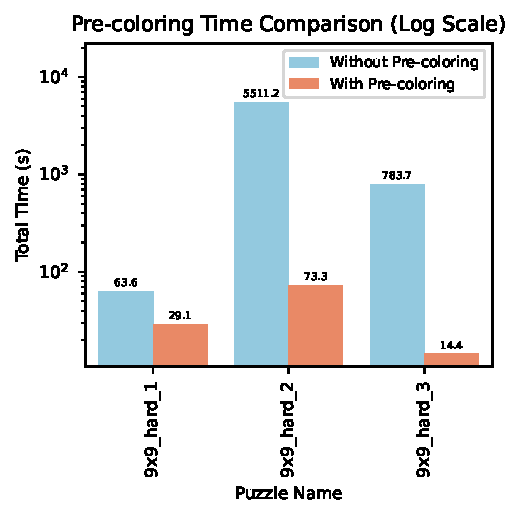
\includegraphics[width=0.9\linewidth]{imgs/precoloring_comparison.pdf}
\caption{Comparison of execution times for some 9x9 futoshiki problems}
\label{fig:precoloring_improvement}
\end{figure}


This figure lets us understand that by employing this technique we can see up to 54x speedup, like in the case of the instance \textit{9x9\_hard\_3}. This means that even if we have a little bit of overhead to apply the list coloring solution, we can still see great improvements over the baseline. For this reason we chose to employ precoloring on all of the following case studies, so that we both reduce the amount of variables in our comparison while introducing several fold speedup in our proposed solution.

\subsection{What the factor are we talking about?}
We have already mentioned that our solutions have a parameter presented as \textit{Configurable Factor}. We said that this factor lets us tweak the ratio between the jobs being scheduled and the underlying computational unit(either a thread for the OpenMP case, or a CPU for the MPI one). From an high level point of view we can think it as a knob that lets us choose at our will the amount of "pressure" that we are putting the underlying system in.

From a more formal point of view, given a factor F and the number of underlying computational units C, our preprocessing algorithm aims at going deeper and deeper into the search space by exploring the backtrack tree until it does not find an amount of puzzles to solve P such that:
\[
    F * C \leq P
\]

This lets us play around to find the best possible ratio, which therefore lets us find the maximum amount of "stress" to put our computational units at before we have generated too many jobs for them.

In fact, we have run several tests to assess which factor could be the best one to choose from, so we now present our \textit{Factor Analysis} that we have devised to pick it.


\begin{figure}[htbp]
\centering
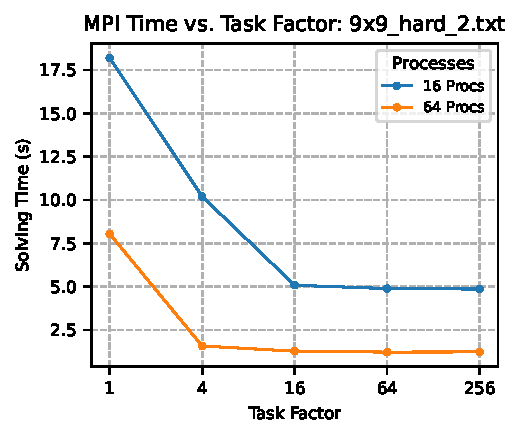
\includegraphics[width=0.9\linewidth]{imgs/factor_mpi_9x9_hard_2.pdf}
\caption{factor analysis for MPI}
\label{fig:factor_analysis_mpi}
\end{figure}

\begin{figure}[htbp]
\centering
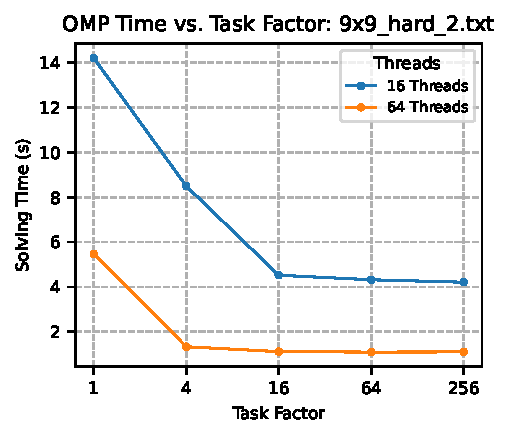
\includegraphics[width=0.9\linewidth]{imgs/factor_omp_9x9_hard_2.pdf}
\caption{factor analysis for OMP}
\label{fig:factor_analysis_omp}
\end{figure}

\begin{figure}[htbp]
\centering
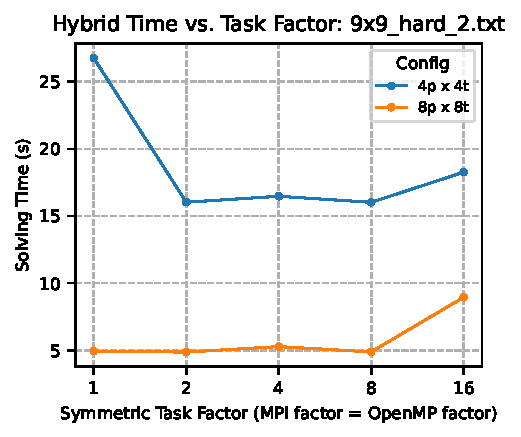
\includegraphics[width=0.9\linewidth]{imgs/factor_hybrid_9x9_hard_2.pdf}
\caption{factor analysis for hybrid solution}
\label{fig:factor_analysis_hybrid}
\end{figure}

From \Cref{fig:factor_analysis_mpi} and \Cref{fig:factor_analysis_omp} we can see that we have a good slope in the decreasing of the solving time of our solution with 16 processors/threads up until 64, and then we start to stabilize. In order to keep things simple, we have opted for this value.

As for the hybrid, we have faced the issue on "how can we evaluate MPI and OMP solutions"? In order to provide some interesting results, we have decided to abstract away from the actual implementation of the worker (MPI or OMP), and we have therefore decided to treat a processor in MPI as the same as the threads for OMP. This modeling simplification is going to help us in \Cref{subsec:hybrid_results} when evaluating how the hybrid solution works under several different configurations.
\sd{check if this link works after doing hybrid results}

After having taken this necessary detour, we can move towards finding the best factor for the hybrid one: we can see from \Cref{fig:factor_analysis_hybrid} that if we consider the symmetric factor 8, which means setting Mpi Factor to 8 and Openmp Factor to 8, if we take this approximation into account (considering processors = threads), we can see how 8*8=64 is also a fairly good factor in this case.


For this reason, we have decided to set for the following runs MPI and OMP factor to 64, and for the hybrid the MPI Factor to 8 and its symmetric counterpart to 8, so that we would have a factor of 64 "computational units" across the board.


\subsection{Parallel Performance Analysis}

After having understood how hard it is to evaluate the difficulty of our problem \textit{a priori}, and having set the ground for our base configuration (hardware used, pre coloring algorithm, factor selected), we can finally move into the evaluation of how our parallel solutions work.

\subsubsection{Solving times for MPI and OMP}
\label{subsubsec:solving_times_mpi_omp}

We start off by showing how our MPI and OMP solutions work with a 9x9\_hard instance and a 10x10\_hard instance (note that the "hard" concept comes from how the website from which we have taken the problems from ranked them. Here are the 2 main sources from which we downloaded \cite{puzzle_futoshiki,puddelbee} and converted images to compatible representation via a custom parser which we have devised in order to gather data).

Please note that as the cluster has a maximum amount of thread per node set to 64, we cannot gather data in the case of 128 threads due to HW constraints. This is the main reason why in the following plots there is not going to be an entry for OMP with 128 Computational units.


We start off by showing a 9x9 instance in \Cref{fig:comparison_solving_time_9x9}. On the x axis we have the number of computational units that we are using, and on the Y axis the time it required for our algorithms to find a valid permutation of numbers to solve the puzzle.

We can see that, as we expect, as the number of computational units increase, the solving time for our problem decreases as we can extract more and more parallel work.

The red dotted line serves as a baseline, as it is the time required for our sequential algorithm to find a solution and it is going to be present in the next graphs also, so that one can easily understand how a given parallel implementation compares w.r.t. the sequential one.

We can see that for 1 and 2 we have values which are in the range of the sequential algorithm minus some seconds of delta in the measurement and this is because, as we have already presented in the \Cref{sec:solution} we have decided to opt for the sequential algorithm to remove the overhead given by OMP and MPI.
\sd{occhio}

\begin{figure}[htbp]
\centering
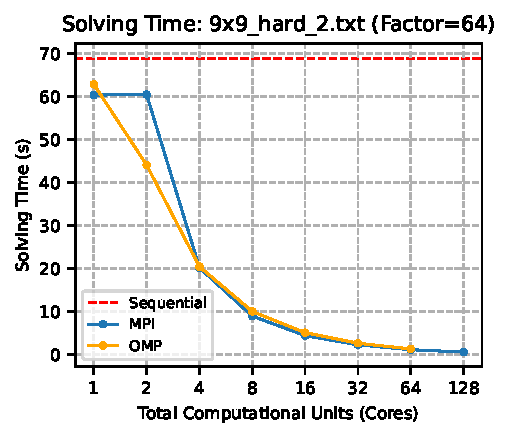
\includegraphics[width=0.9\linewidth]{imgs/solving_time_mpi_omp_9x9_hard_2.pdf}
\caption{Solving time comparison for a 9x9 instance}
\label{fig:comparison_solving_time_9x9}
\end{figure}

We now move towards a 10x10 instance. In \Cref{fig:comparison_solving_time_10x10} we see something strange: every parallel implementation is consistently worse w.r.t. solving time compared to the sequential solution (minus some cases like the 4,8 and 16 CU which have little to no actual increase in performance). 

This is very interesting, because by looking at the absolute value of the solving time we can note that even the sequential algorithm is taking less than 0.01 second to find the solution. This lets us draw two necessary conclusions:
\begin{enumerate}
    \item As we have stated in \Cref{subsec:futoshiki_difficulty}, the size alone is not a factor which directly implies the difficulty of the problem. We can see that the absolute time to solve the 9x9 and 10x10 are vastly different, even if someone might at a first glance say "if we have more cells we should have higher execution times". This does not always hold if we do not consider all of the aforementioned variables.
    \item Parallel solutions introduce some overhead, either the message passing infrastructure needed for the MPI framework to process messages, or the locks needed to achieve high efficiency shared memory reading and writing when accessing critical parts of code. Such overhead is usually mitigated by the fact that the overall performance increase in finding a solution is higher than the overhead introduced by parallelizing the work. This is not the case for these specific families of problems: as the sequential solution is already extremely fast, it does not make sense to parallelize it, and therefore we can conclude that this family of instances are not tailored or our parallel solution analysis.
\end{enumerate}

For such reasons, we are going to move to analyze only the family of 9x9 instances, as they are more interesting and actually give us some interesting data and points to reason about w.r.t. just saying "for the 10x10 instance we have a degradation in performance".

\begin{figure}[htbp]
\centering
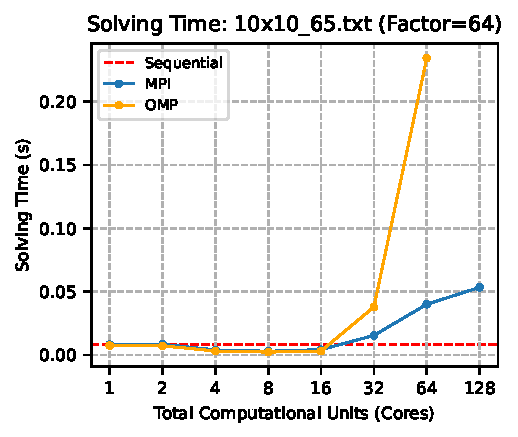
\includegraphics[width=0.9\linewidth]{imgs/solving_time_mpi_omp_10x10_65.pdf}
\caption{Solving time comparison for a 10x10 instance}
\label{fig:comparison_solving_time_10x10}
\end{figure}

\subsubsection{How well does parallel solution perform compared to sequential?}
\label{subsubsec:speedup_efficiency}

Now that the reader has understood how configurations and difficulty of the puzzles impact the overall execution time, he might ask himself "is there a metric to evaluate how much better the parallel solutions are compared to the sequential one?"

Turns out that we have such metrics. We know that if we have a task and we parallelize it, we can use the \textit{Speedup} concept to understand how much better it gets, and it is presented as:
\[
S = \frac{Execution\_time\_sequential}{Execution\_time\_parallel}
\]
This means that the lower the execution time is when parallelized, the higher the speedup is going to be. In \Cref{fig:speedup_9x9} we show the speedup that we can reach with our solution. On the x axis w.h. the computational units, whereas in the Y axis we have the speedup value. The red line represents the theoretical speedup that we can reach, so assuming that the parallelization of the task introduces absolutely 0 overhead.

An interesting takeaway from this plot is that while we reach a speedup which is close to the ideal one in the 0-20 computational units case, we can see how by increasing the number of units we have a speedup value which does not grow as fast as the theoretical one. From this we can conclude that:
\begin{enumerate}
    \item As the number of computational units increase, we introduce higher overhead due to the message passing or the shared variables accesses, which is not much if we have "few" computational units, but as the number goes up the overhead is getting a little bit bigger, therefore impacting the overall speedup.
    \item The fact that the speedup does not grow as fast as the ideal one does not mean that the solution gets slower: It is still faster than the sequential solution.
\end{enumerate}


\begin{figure}[htbp]
\centering
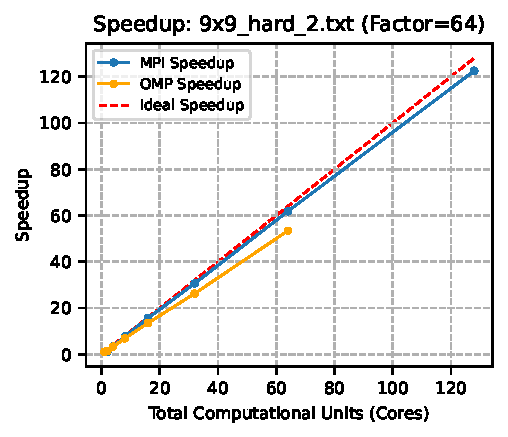
\includegraphics[width=0.9\linewidth]{imgs/speedup_mpi_omp_9x9_hard_2.pdf}
\caption{Speedup of parallel solutions}
\label{fig:speedup_9x9}
\end{figure}

We can now move into the second metric that we can use to evaluate our parallel algorithm w.r.t. the sequential one: the \textit{Efficiency}. This is a derivative parameter which is dependent on the speedup, and it can be expressed as:
\[
E = \frac{Speedup}{\# computational\_units}
\]

This parameter is basically relating the speedup(how well the parallel solution is w.r.t. the sequential one) with the number of units available. This parameter is therefore going to tell us how well the available cores are being used.

\Cref{fig:efficiency_9x9} we can see how efficiency is evaluated in our solutions. We see how the overall efficiency decreases as the number of computational units increase. This is expected: efficiency is a mirror of the speedup, so as we have noticed how that was decreasing due to the overhead of the underlying technologies used, we should expect that the amount of work to be done is going to decrease as the amount of available computational cores increases. We can however note that 
\begin{enumerate}
    \item OMP is strictly dominating the MPI efficiency plot, and this tells us that OMP overhead due to the shared memory access is stricly lower than the message passing approach used by MPI, which is fairly interesting. 
    \item We have a high decrease in efficiency when increasing the number of cores from 1 to 2,4 but then we stabilize as the number of core increases. This is expected as, since the efficiency explains how much each core is contributing and "kept busy" to achieve the final goal, as we increase the amount of available cores we give less amount of work to every core which is expected.
\end{enumerate}
\sd{we can say in future works play with factor to see how to maximize efficiency of solution which is good!}

\begin{figure}[htbp]
\centering
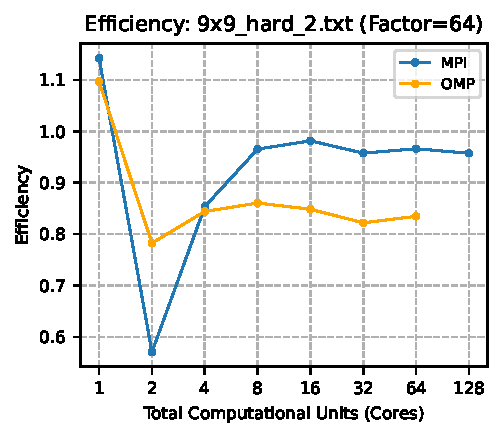
\includegraphics[width=0.9\linewidth]{imgs/efficiency_mpi_omp_9x9_hard_2.pdf}
\caption{Efficiency of parallel solutions}
\label{fig:efficiency_9x9}
\end{figure}




\subsubsection{MPI Scalability}
Table \ref{tab:mpi_scaling} presents MPI performance across multiple nodes:

\begin{table}[htbp]
\caption{MPI Strong Scaling (9×9 Hard Puzzle)}
\begin{center}
\begin{tabular}{@{}ccccc@{}}
\toprule
\textbf{Processes} & \textbf{Time (s)} & \textbf{Speedup} & \textbf{Efficiency} \\
\midrule
1 & 35.84 & 1.00 & 100.0\% \\
2 & 18.21 & 1.97 & 98.5\% \\
4 & 9.45 & 3.79 & 94.8\% \\
8 & 5.11 & 7.01 & 87.6\% \\
16 & 3.02 & 11.87 & 74.2\% \\
32 & 2.25 & 15.93 & 49.8\% \\
64 & 2.05 & 17.48 & 27.3\% \\
128 & 2.01 & 17.83 & 13.9\% \\
\bottomrule
\end{tabular}
\end{center}
\label{tab:mpi_scaling}
\end{table}

MPI maintains higher efficiency than OpenMP at moderate scales due to better memory locality, but communication overhead becomes significant beyond 32 processes.

\subsubsection{OpenMP Scalability}
Table \ref{tab:openmp_scaling} shows OpenMP performance with increasing thread counts on a single node:

\begin{table}[htbp]
\caption{OpenMP Strong Scaling (9×9 Hard Puzzle)}
\begin{center}
\begin{tabular}{@{}ccccc@{}}
\toprule
\textbf{Threads} & \textbf{Time (s)} & \textbf{Speedup} & \textbf{Efficiency} \\
\midrule
1 & 35.84 & 1.00 & 100.0\% \\
2 & 18.45 & 1.94 & 97.2\% \\
4 & 9.78 & 3.67 & 91.7\% \\
8 & 5.42 & 6.61 & 82.6\% \\
16 & 3.18 & 11.27 & 70.4\% \\
32 & 2.36 & 15.19 & 47.5\% \\
64 & 2.35 & 15.25 & 23.8\% \\
\bottomrule
\end{tabular}
\end{center}
\label{tab:openmp_scaling}
\end{table}

OpenMP shows excellent efficiency up to 8 threads, with diminishing returns beyond 16 threads due to NUMA effects and increased synchronization overhead.


\subsubsection{Hybrid Performance}
The hybrid solver demonstrates superior scalability by combining both paradigms:

\begin{table}[htbp]
\caption{Hybrid Scaling with Various Configurations (11×11 Hard Puzzle)}
\begin{center}
\begin{tabular}{@{}cccccc@{}}
\toprule
\textbf{MPI} & \textbf{OMP} & \textbf{Total} & \textbf{Time} & \textbf{Speedup} \\
\textbf{Procs} & \textbf{Threads} & \textbf{Cores} & \textbf{(s)} & \\
\midrule
1 & 1 & 1 & 142.36 & 1.00 \\
1 & 4 & 4 & 37.82 & 3.76 \\
2 & 2 & 4 & 36.94 & 3.85 \\
4 & 1 & 4 & 38.45 & 3.70 \\
2 & 8 & 16 & 10.28 & 13.85 \\
4 & 4 & 16 & 9.87 & 14.42 \\
8 & 2 & 16 & 10.95 & 13.00 \\
4 & 16 & 64 & 5.12 & 27.80 \\
8 & 8 & 64 & 5.03 & 28.31 \\
16 & 4 & 64 & 5.38 & 26.46 \\
\bottomrule
\end{tabular}
\end{center}
\label{tab:hybrid_scaling}
\end{table}

The hybrid approach achieves the best overall speedup (28.3×) by effectively utilizing both parallelization levels. The 8×8 configuration (8 MPI processes with 8 OpenMP threads each) provides optimal performance for 64 cores.

\subsection{Task Generation Factor Analysis}
We investigated the impact of the task generation factor—a multiplier that controls work unit granularity. Figure \ref{fig:task_factor} shows performance variation with different factors:

\begin{figure}[htbp]
\centering
\includegraphics[width=0.9\linewidth]{images/precoloring }
\caption{Performance impact of task generation factor for 64 cores. Optimal performance occurs around factor = 4-8.}
\label{fig:task_factor}
\end{figure}

Optimal performance occurs around factor = 4-8, balancing sufficient parallelism against overhead. Lower factors cause load imbalance, while higher factors increase coordination overhead.

\subsection{Weak Scaling Analysis}
To evaluate scalability with increasing problem size, we conducted weak scaling experiments where puzzle size grows proportionally with processor count:

\begin{table}[htbp]
\caption{Weak Scaling Efficiency}
\begin{center}
\begin{tabular}{@{}ccccc@{}}
\toprule
\textbf{Cores} & \textbf{Puzzle} & \textbf{Time (s)} & \textbf{Efficiency} \\
\midrule
1 & 5×5 & 0.23 & 100.0\% \\
4 & 7×7 & 0.31 & 92.7\% \\
16 & 9×9 & 0.45 & 87.3\% \\
64 & 11×11 & 0.68 & 79.4\% \\
\bottomrule
\end{tabular}
\end{center}
\label{tab:weak_scaling}
\end{table}

The solver maintains good weak scaling efficiency, demonstrating its ability to handle larger problems with proportionally more resources.

\subsection{Performance Summary}
Figure \ref{fig:speedup_comparison} summarizes the speedup achieved by each implementation:

\begin{figure}[htbp]
\centering
\includegraphics[width=0.9\linewidth]{images/speedup_chart.png}
\caption{Speedup comparison across all implementations. The hybrid approach consistently outperforms single-paradigm solutions.}
\label{fig:speedup_comparison}
\end{figure}

Key observations:
\begin{itemize}
    \item \textbf{Sequential Optimization:} Pre-coloring provides 14× speedup, essential for all parallel versions
    \item \textbf{Shared Memory:} OpenMP excels within a single node but plateaus at 32 threads
    \item \textbf{Distributed Memory:} MPI scales better across nodes but has higher communication overhead
    \item \textbf{Hybrid Approach:} Combines strengths of both paradigms, achieving best overall performance
\end{itemize}
\section{Conclusion}
\label{sec:conclusion}
We presented a comprehensive high-performance computing implementation for solving the Futoshiki puzzle, demonstrating the feasibility of solving an instance of an NP-hard by employing several different techniques, starting from the search space reduction via precoloring, and later on moving towards MPI, OMP and Hybrid solutions.

We have to note that when gathering data from the runs, we have noticed some discrepancies w.r.t. the execution times, and this is most likely dependent from the fact that older machine with the same node category (c-nodes) might have different hardware, or there is some wear and tear damage performed. Another factor is also due to the fact that the scheduler and the timing of when some jobs are scheduled might incur in some variance over the expected finishing time of our solutions.

\subsection{Key Achievements}
Our implementation achieves significant performance improvements at multiple levels:

\begin{enumerate}
    \item \textbf{Algorithmic Optimization:} We have seen that pre-coloring phase, based on list coloring theory, reduces the search space by 70-90\%, providing a 59× speedup over naive backtracking. This optimization is crucial for making puzzles which have a bigger search space tractable also with a sequential solution, and therefore we opted to apply in every subsequent experiment.
    
    \item \textbf{Parallel Scalability:} We successfully parallelized the solver using three distinct paradigms. Here are the execution time findings:
    \begin{itemize}
        \item \textbf{OpenMP} achieves up to 53.4× speedup on 64 threads with minimal code complexity compared to the sequential solution.
        \item \textbf{MPI} demonstrates 123× speedup when using 128 processes. From our Speedup analysis it also slightly beat the OMP solution and therefore was also the best for the efficiency parameter. This means that, while the OMP solution is the easier one to implement compared to the MPI version, it also suffers more from memory contention and mutex or lock-like structures needed to perform syanchronization.
        \item \textbf{Hybrid MPI+OpenMP} reaches 60.4× speedup when using 32 CPUs and 8 threads, which showcases how leveraging MPI is actually the best solution compared to the other hybrid configurations. This was expected as the MPI only solution is already slightly better than OMP. An interesting finding is that while the Hybrid does not perform as good as the MPI only overall, there are still cases in which its configurability can lead to better results compared to our test under analysis.
    \end{itemize}
    
    \item \textbf{Dynamic Work Generation:} Our unified framework automatically adjusts work unit granularity based on available parallelism, ensuring efficient resource utilization across different scales and architectures.
    \sd{this seems too vague but idk what to say}
    
    \item \textbf{Configurable Performance:} The task generation factor allows fine-tuning for specific hardware configurations and puzzle characteristics, with 64 factor leading up to \textbf{3.5x} speedup over the baseline (factor set to 1, which means we are not oversubscribing anything).

    \item \textbf{Scalability Analysis}: the Strong analysis lead us to understanding that MPI achieves almost linear speedups and retains higher efficiency, making it the best solution if we are aiming at maximizing that parameter. We have also seen that, due to the fact that it is hard to determine a priori how complex a puzzle can be to solve given only its size, it does not make sense to proceed with the Weak scalability analysis.
\end{enumerate}


Overall we can therefore say that the speedup performed by the list coloring algorithm in order to precolor the solution is extremely important, that in our evaluated instance MPI outperforms OMP and the hybrid solution, while at times it introduces some overhead due to the message passing and shared memory synchronization, therefore decrementing the efficiency at higher computational units selected, still serves as a fairly interesting solution due to its extreme configurability. This does not mean that the OMP solution is bad as a whole, what we are stating is that the other two solutions outperform it, but still is an extremely useful entrypoint due to its ease of implementation, as it requires little work to transform some sequential algorithms to parallel ones.


\subsection{Technical Contributions}
Beyond solving Futoshiki puzzles, our work makes several contributions to parallel computing for constraint satisfaction problems:

\begin{itemize}
    \item \textbf{Modular Design:} The separation of work generation, distribution, and solving enables easy adaptation to other CSP problems
    \item \textbf{Scalability Analysis:} Comprehensive evaluation of strong and weak scaling provides insights into parallel efficiency limits
    \item \textbf{Hybrid Methodology:} Demonstrates effective combination of MPI and OpenMP for irregular workloads
    \item \textbf{Performance Portability:} Implementation runs efficiently from single-core laptops to large HPC clusters
\end{itemize}
\section{Future Work}
\label{sec:future_work}
During the course of this report we have presented how our framework compares w.r.t. a standard sequential solution when it comes to the instance of Futoshiki solving. 

There are still some areas to explore in order to shed some light into. Here are presented in a bullet point fashion:

\subsection{Algorithmic Enhancements}
\begin{itemize}
    \item \textbf{Variable Ordering Heuristics:} Implement most-constrained-variable (MCV) and minimum-remaining-values (MRV) heuristics to select cells more intelligently during backtracking.
    
    \item \textbf{Arc Consistency:} Extend constraint propagation to AC-3 or higher levels of consistency for more aggressive pruning.
    \sd{dunno what this is, maybe we can remove}
    
    \item \textbf{Optimizing search space reduction:} We have seen how the precoloring algorithm already does some of the heavy lifting when it comes to reducing the search space, but there are still some techniques which can be applied. The first one would be to  Implement \textit{clause learning} to avoid redundant exploration of similar subtrees, which can happen quite frequently considering the class of search space. The latter technique is the \textit{Symmetry Breaking}, which conceptually is similar to the Symmetry Breaking (as of we aim to remove already found patterns).
    
    \item \textbf{Parameter tweaking}: We have seen how the Hybrid configuration enables some configuratbility by defining how much the solution can rely on MPI or OMP, we can therefore move in this direction to tweak these parameters and see how hybrid solution works in different scenarios.

    Another \textit{factor }to play around with is the configuration factor itself. As it determines the amount of over subscription, playing around with this value could lead to interesting findings in its relation with the \textit{efficiency}.
    \sd{maybe?}
    \item \textbf{Reducing communication overhead} via non-blocking MPI message passing strategies, which would lead to a decrease of idle-time in the single CPUs.

    \item \textbf{A new metric}: we have stated that it is not easy to determine the complexity of a problem based on single variables alone (e.g. size, number of constraints, etc). As this goes beyond the scope of exploring the parallelization of this problem, we have still decided to include this bullet point as by finding a single metric which takes into account all of the variables of the problem in one go, one could design a configuration finder such that, given the puzzle, it would find the best configuration(either in the hybrid zone, or just picking OMP or MPI for some specific tasks) to enhance the performance of the whole solution.

    \item \textbf{Distributed Precoloring}: while we have stated that due to the law of deminishing returns it does not make much sense to distribute the first precoloring phase, given a huge search space the overhead of parallelizing also this problem could be a smaller factor compared to the time taken for our current sequential precoloring algorithm, so this might be worth exploring in the future.
    \item \textbf{More dynamic structure}: by collecting runtime data, one could implement a more dynamic work distribution.
\end{itemize}

These extensions would further improve performance, increment the applicability area of our solution, and make the framework more accessible to researchers working on constraint satisfaction problems or instances which can be easily reduced to CSPs.
\section{Related Work}
Our work builds upon and extends research in several areas: constraint satisfaction algorithms, parallel computing for combinatorial problems, and puzzle-solving techniques.

\subsection{Constraint Satisfaction and Propagation}
The foundation of our approach lies in constraint propagation techniques. Norvig's influential work on Sudoku solving \cite{NorvigSudoku} demonstrated the power of constraint propagation combined with search, achieving dramatic speedups over naive backtracking. Our pre-coloring phase extends these ideas specifically for Futoshiki's inequality constraints.

The transformation of Futoshiki into a list coloring problem, as proposed by Şen and Diner \cite{Sen2024Futoshiki}, provides the theoretical foundation for our implementation. Their work showed that viewing the puzzle through the lens of graph coloring enables more sophisticated pruning strategies. We extend their sequential algorithm with parallel execution while preserving the correctness guarantees.

Colbourn's seminal work \cite{Colbourn1984} on the complexity of Latin Square completion established the NP-completeness of the problem class, motivating the need for efficient heuristics and parallel approaches. Haraguchi and Ono \cite{Haraguchi2014} further analyzed the approximability of Latin Square completion puzzles, providing insights into the theoretical limits of polynomial-time algorithms.

\subsection{Parallel Backtracking and Search}
Parallel constraint satisfaction has been extensively studied, with various approaches proposed for distributing the search space. The book by Pacheco \cite{Pacheco2011} provides comprehensive coverage of parallel programming patterns, including the master-worker paradigm we employ. However, most existing work uses static work distribution, whereas our dynamic multi-level approach better handles the irregular search space of Futoshiki.

Research on parallel backtracking typically focuses on either shared-memory or distributed-memory systems in isolation. Our contribution lies in effectively combining both paradigms and demonstrating that hybrid approaches can outperform single-paradigm solutions for irregular workloads.

\subsection{MPI and OpenMP for Irregular Problems}
The MPI standard \cite{MPIForum2021} and OpenMP specification \cite{OpenMP2020} provide the foundation for our parallel implementations. Gropp et al. \cite{Gropp1999} discuss various MPI programming patterns, including the master-worker model we adapt for dynamic load balancing.

Rabenseifner et al. \cite{Rabenseifner2009} specifically address hybrid MPI/OpenMP programming, analyzing the benefits and challenges of combining both paradigms. Their work on multi-core clusters directly influenced our hybrid implementation design. We extend their findings by demonstrating that careful management of task generation factors at both levels is crucial for optimal performance.

\subsection{Puzzle Solving Algorithms}
Beyond Sudoku, various researchers have tackled different puzzle types with parallel algorithms. The general approach of combining constraint propagation with parallel search has proven effective across multiple domains. However, most work focuses on puzzles with uniform constraints (like Sudoku's boxes), whereas Futoshiki's arbitrary inequality constraints present unique challenges.

Our work differs from existing puzzle solvers in several key aspects:
\begin{itemize}
    \item \textbf{Multi-paradigm approach:} We systematically compare three parallelization strategies
    \item \textbf{Dynamic depth calculation:} Our work generation adapts to both puzzle difficulty and available parallelism
    \item \textbf{Configurable granularity:} The task factor mechanism allows performance tuning without code changes
    \item \textbf{Comprehensive evaluation:} We provide detailed analysis of both strong and weak scaling
\end{itemize}

\subsection{Load Balancing in Parallel Computing}
Load balancing for irregular problems remains an active research area. Static approaches suffer from load imbalance when work units have varying difficulty, while dynamic approaches incur communication overhead. Our solution strikes a balance by generating sufficient work units upfront (based on the calculated depth) while using on-demand distribution to handle variability.

The concept of oversubscription—creating more tasks than workers—is well-established in parallel computing. Our contribution is the systematic study of the task generation factor's impact on performance, showing that 4-8× oversubscription optimally balances parallelism with overhead for constraint satisfaction problems.

\subsection{High-Performance Computing for AI}
The intersection of HPC and artificial intelligence has gained significant attention. While much focus is on machine learning, combinatorial optimization and constraint satisfaction remain important applications. Our work demonstrates that traditional AI techniques like backtracking can benefit substantially from modern parallel computing infrastructure.

The scalability results we achieve (up to 28× speedup on 64 cores) are competitive with other parallel constraint solvers, while our modular design facilitates adaptation to other problems. This positions our framework as a valuable contribution to both the HPC and AI communities.

% Bibliography
\bibliographystyle{IEEEtran}
\bibliography{bibliography}

\end{document}
